% Bản nháp độc lập: chuyển nội dung sang template chính thức khi có.
% Biên dịch bằng XeLaTeX từ thư mục gốc: xelatex -output-directory=report report/report.tex
\documentclass[11pt,a4paper]{article}
\usepackage{fontspec}
\usepackage{polyglossia}
\setdefaultlanguage{vietnamese}
\usepackage{geometry,graphicx,booktabs,hyperref,float}
\geometry{margin=2.5cm}
\title{FIT4013 -- Dự đoán sinh viên có nguy cơ bỏ học\\\large Bản nháp báo cáo, chưa theo template học phần}
\author{Nhóm: bổ sung danh sách và phân công thực tế}
\date{}
\begin{document}
\maketitle
\section{Đặt vấn đề và phân tích yêu cầu}
Mục tiêu là dự đoán tại thời điểm nhập học ba trạng thái cuối thời hạn khóa học: Dropout, Enrolled, Graduate. Kết quả là tín hiệu để nhân viên xem xét hỗ trợ, không phải quyết định tự động. Theo UCI, dữ liệu từ một cơ sở giáo dục đại học, gồm thông tin lúc nhập học và kết quả học kỳ 1--2; nhãn ghi trạng thái cuối thời hạn chuẩn khóa học \cite{uci}. Bài toán ba lớp theo dữ liệu gốc; Enrolled không đồng nghĩa chắc chắn sẽ bỏ học sau này.

Tệp gốc gồm 4.424 dòng, 36 đặc trưng và một nhãn; dấu phân cách chấm phẩy; không có ô trống hay dòng trùng hoàn toàn. Dropout 1.421 (32,1\%), Enrolled 794 (17,9\%), Graduate 2.209 (49,9\%). Trong tập train 3.539 dòng, tuổi nhập học trung vị 20, tứ phân vị 19--25, khoảng 17--70. Theo quy tắc 1,5 IQR, tuổi có 358 giá trị ngoại lệ, thứ tự nguyện vọng 431, điểm văn bằng trước 135, điểm tuyển sinh 68. Các giá trị này không tự chứng minh lỗi và không bị xóa. Mã ngành là mã phân loại, không phải thang số. Thống kê, tần suất từng biến phân loại, ma trận tương quan số và các biểu đồ nằm trong \texttt{results/}; xem Hình~\ref{fig:eda}. UCI cho biết dữ liệu đã được xử lý bất thường và thiếu trước khi công bố, nên việc không có ô trống không phản ánh nhất thiết dữ liệu gốc chưa xử lý.
\begin{figure}[H]\centering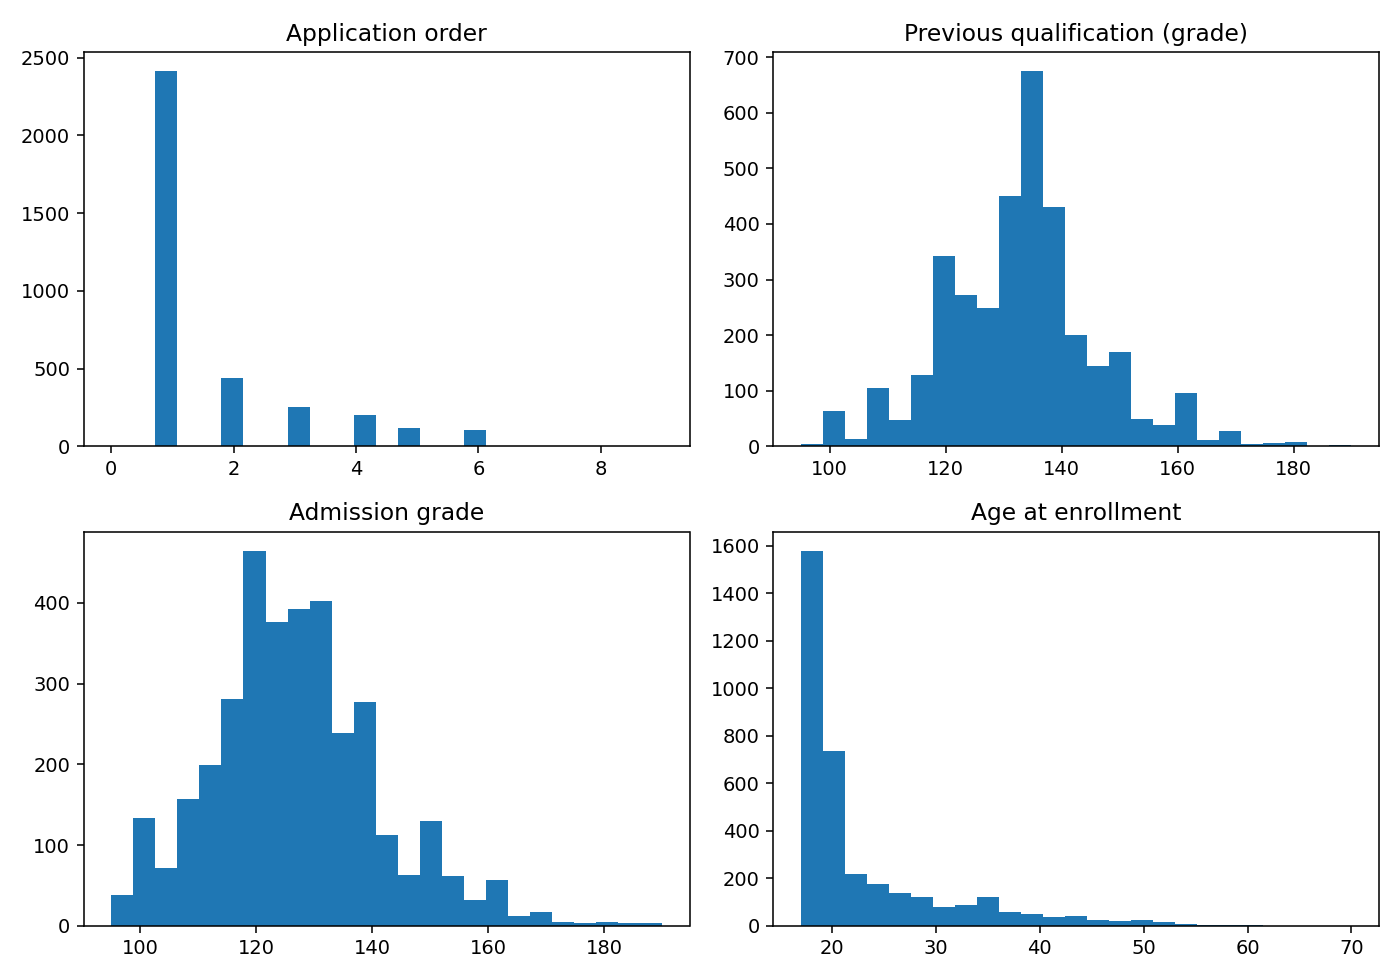
\includegraphics[width=.7\textwidth]{results/eda_histograms.png}\caption{Phân phối đặc trưng số trên tập train.}\label{fig:eda}\end{figure}

\section{Thiết kế giải pháp và quy trình học máy}
Quy trình: CSV $\rightarrow$ kiểm tra schema $\rightarrow$ chia phân tầng $\rightarrow$ 5 fold train, học tiền xử lý trong mỗi fold $\rightarrow$ chọn tham số theo macro-F1 $\rightarrow$ huấn luyện lại trên train $\rightarrow$ đánh giá test cố định. Seed 42; chia 80/20 được UCI khuyến nghị. Mọi tổ hợp dùng cùng 3.539 dòng train, 885 dòng test và cùng các fold; chỉ số dòng được lưu.

Danh sách cho phép gồm 18 biến: thứ tự nguyện vọng, điểm văn bằng trước, điểm tuyển sinh, tuổi lúc nhập học; tình trạng hôn nhân, hình thức đăng ký, ngành học, ca học, văn bằng trước, quốc tịch, trình độ và nghề của cha mẹ, chuyển nơi ở, nhu cầu giáo dục đặc biệt, giới tính và sinh viên quốc tế. UCI mô tả dữ liệu gồm thông tin tại nhập học nhưng không xác nhận dấu thời gian từng trường: displaced, nhu cầu đặc biệt và thông tin gia đình cần kiểm chứng trong hệ thống thực. Không dùng 12 kết quả hai học kỳ; loại nợ, học phí, học bổng do thời điểm chốt không rõ, cũng như ba chỉ số kinh tế vĩ mô do không rõ thời điểm công bố. Không coi tương quan là quan hệ nhân quả.

Cả hai luồng dùng median cho số, mode và one-hot cho phân loại, cho phép mã chưa thấy; không có dữ liệu thiếu ở tệp này nhưng bước dự phòng vẫn chỉ học từ train. Luồng A baseline dùng StandardScaler; B thay duy nhất bằng RobustScaler (median/IQR). Giả thuyết: B giảm ảnh hưởng giá trị ngoại lệ lên khoảng cách K-NN, nhưng có thể làm thay đổi trọng số tương đối của đặc trưng. Cây quyết định chia theo ngưỡng, nên về nguyên tắc ít nhạy với các phép biến đổi đơn điệu; sai số số thực và điểm hòa có thể tạo chênh lệch nhỏ.

K-NN dùng khoảng cách Minkowski mặc định và thử $k=3,5,11,21,31$; cây dùng Gini mặc định với độ sâu $3,5,8,12$ và không giới hạn. Hai thuật toán có giả định khác nhau: khoảng cách lân cận phụ thuộc thang đo và số chiều one-hot; cây dễ diễn giải cục bộ nhưng có thể quá khớp. Macro-F1 cân bằng tầm quan trọng ba lớp; dropout recall được ghi riêng. Chọn theo macro-F1 trung bình trên năm fold, không tối ưu theo test.

\section{Phân tích mã nguồn và chức năng}
\texttt{data.py} kiểm định cột, nhãn và kiểu số, kiểm kê và chia dữ liệu; \texttt{preprocess.py} xây dựng hai ColumnTransformer; \texttt{train.py} tạo EDA, các fold, tìm kiếm lưới và log; \texttt{evaluate.py} xuất metric, nhãn dự đoán và ma trận nhầm lẫn. \texttt{scripts/download\_data.py} tải CSV chính thức, \texttt{results/} chứa kết quả và chỉ số dòng để kiểm tra khả năng tái lập. Mã tiền xử lý nằm bên trong pipeline của GridSearchCV.

\section{Thử nghiệm và kết quả}
Bảng \ref{tab:cv} là macro-F1 trung bình năm fold; chi tiết điểm từng fold và recall Dropout có trong các tệp \texttt{*\_cv.csv}. Các tham số chọn: A/K-NN $k=11$, B/K-NN $k=5$, cả hai cây độ sâu 12.
\begin{table}[H]\centering\small
\begin{tabular}{lrrrrr}\toprule
K-NN ($k$) & 3 & 5 & 11 & 21 & 31\\\midrule
A & .4222 & .4401 & .4432 & .4212 & .4129\\
B & .4206 & .4467 & .4410 & .4223 & .4133\\\midrule
Cây (độ sâu) & 3 & 5 & 8 & 12 & không giới hạn\\\midrule
A & .4130 & .4200 & .4277 & .4347 & .4241\\
B & .4130 & .4200 & .4277 & .4347 & .4254\\\bottomrule
\end{tabular}\caption{So sánh siêu tham số trên train.}\label{tab:cv}\end{table}
\begin{table}[H]\centering\small
\begin{tabular}{llrrrrr}\toprule
Luồng & Mô hình & Accuracy & P macro & R macro & F1 macro & R Dropout\\\midrule
A & K-NN & .5571 & .4589 & .4439 & .4326 & .4472\\
A & Cây & .5345 & .4681 & .4608 & .4620 & .4789\\
B & K-NN & .4949 & .3909 & .4006 & .3919 & .4437\\
B & Cây & .5345 & .4681 & .4608 & .4620 & .4789\\\bottomrule
\end{tabular}\caption{Kết quả trên cùng 885 mẫu test; P/R là precision/recall.}\label{tab:test}\end{table}
\begin{table}[H]\centering\small
\begin{tabular}{llrrrr}\toprule
Tổ hợp & Lớp & Precision & Recall & F1 & Số mẫu\\\midrule
A K-NN & Dropout & .5292 & .4472 & .4847 & 284\\
 & Enrolled & .2500 & .0881 & .1302 & 159\\
 & Graduate & .5976 & .7964 & .6828 & 442\\\midrule
A/B Cây & Dropout & .4964 & .4789 & .4875 & 284\\
 & Enrolled & .2941 & .2201 & .2518 & 159\\
 & Graduate & .6138 & .6833 & .6467 & 442\\\midrule
B K-NN & Dropout & .4437 & .4437 & .4437 & 284\\
 & Enrolled & .1429 & .0818 & .1040 & 159\\
 & Graduate & .5863 & .6765 & .6282 & 442\\\bottomrule
\end{tabular}\caption{Chỉ số từng lớp trên test.}\end{table}
\begin{figure}[H]\centering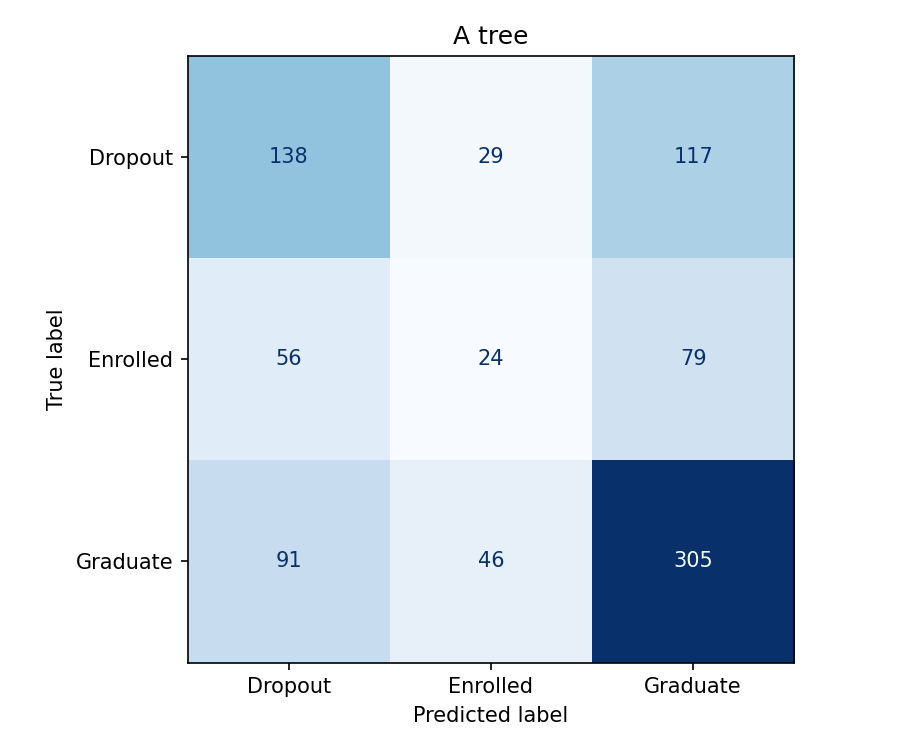
\includegraphics[width=.65\textwidth]{results/A_tree_confusion_matrix.png}\caption{Ma trận nhầm lẫn cây luồng A: hàng là nhãn thật, cột là dự đoán.}\end{figure}
\begin{figure}[H]\centering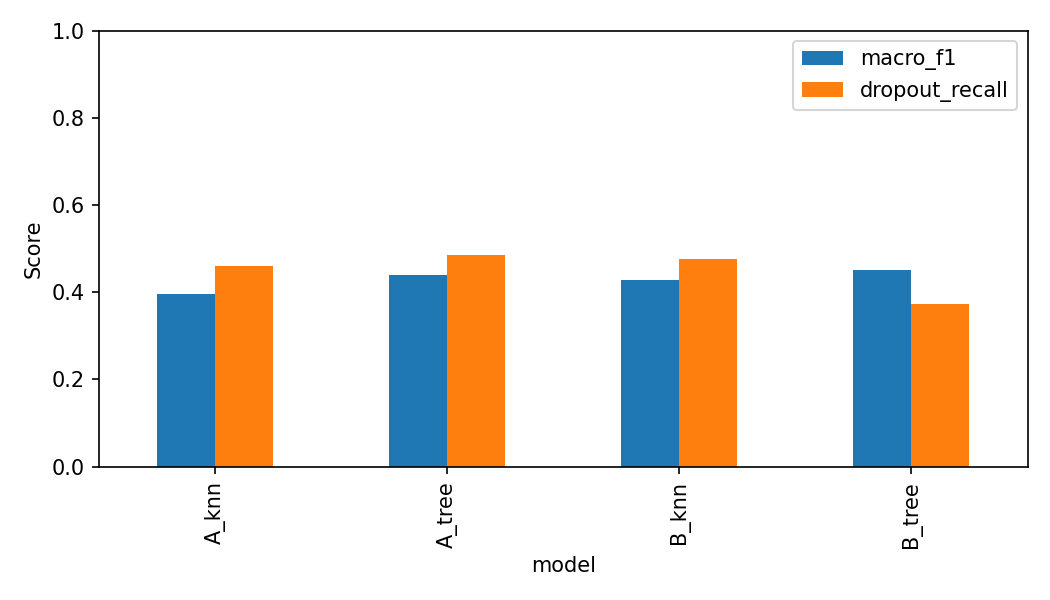
\includegraphics[width=.65\textwidth]{results/comparison.png}\caption{So sánh macro-F1 và recall Dropout.}\end{figure}

\section{Thảo luận và so sánh}
Ở test, cây A và B cùng dự đoán và đạt macro-F1 .4620; K-NN A đạt .4326 còn B .3919. B không cải thiện K-NN trên lần chia này, dù CV của B cao hơn A một chút (.4467 so với .4432); chưa thể suy ra tác động ổn định vì chỉ có một test split và các cấu hình K-NN được chọn khác nhau. Cây có cùng dự đoán test dù điểm CV hơi khác; tính bất biến của ngưỡng và sai số số thực là lời giải thích hợp lý, không phải bằng chứng nhân quả.

Ở cây A/B, trong 284 Dropout thật, 148 bị bỏ sót: 38 dự đoán Enrolled và 110 Graduate; 44 trong 159 Enrolled bị nhầm thành Dropout. Recall Enrolled chỉ .2201. Ở A K-NN có 157 Dropout bị bỏ sót (21 Enrolled, 136 Graduate); 44 Enrolled bị nhầm Dropout. Ở B K-NN có 158 bỏ sót (33 Enrolled, 125 Graduate) và 60 Enrolled nhầm Dropout. \texttt{*\_predictions.csv} lưu từng trường hợp bằng chỉ số dòng; không công bố thêm thuộc tính cá nhân của các ví dụ. Khả năng phân biệt Enrolled kém có thể liên quan mất cân bằng và thông tin nhập học hạn chế, nhưng chưa được kiểm chứng là nguyên nhân. Các dự đoán sai có thể bỏ sót hỗ trợ hoặc tạo cảnh báo không cần thiết.

Tập dữ liệu một cơ sở, chưa có kiểm định theo thời gian, trường khác, độ công bằng theo nhóm hay khoảng tin cậy; split ngẫu nhiên có thể đánh giá lạc quan khi triển khai theo các khóa tương lai. Sau khi xem test, mọi điều chỉnh cần bộ kiểm định độc lập mới. Một số biến nhân khẩu nhạy cảm cần đánh giá tính hợp pháp, công bằng và sự cần thiết trước khi sử dụng thực tế.

\section{Tổng kết và hướng phát triển}
Cây đạt macro-F1 test cao nhất trong bốn tổ hợp nhưng bỏ sót hơn một nửa Dropout; chưa đủ tin cậy để dùng độc lập. Bước tiếp theo: xác nhận thời điểm thu thập từng biến, đánh giá theo khóa nhập học, trường và nhóm dân số; thử trọng số lớp hoặc ngưỡng cảnh báo trong train, rồi đánh giá trên test mới. Đánh giá lợi ích, chi phí nhân sự và tác động sai lệch cùng nhà trường trước triển khai.

\appendix
\section{Khai báo sử dụng AI}
OpenAI Codex được dùng để hỗ trợ đọc hướng dẫn, thiết kế và viết mã, chạy thí nghiệm, sửa lỗi và soạn bản nháp. Các số liệu lấy từ lần chạy thực tế. Nhóm cần kiểm tra và chịu trách nhiệm về toàn bộ nội dung, khai báo thêm các sử dụng AI khác nếu có và bổ sung phân công thực tế.
\begin{thebibliography}{9}
\bibitem{uci} V. Realinho, M. V. Martins, J. Machado, L. Baptista (2021), \emph{Predict Students' Dropout and Academic Success}, UCI Machine Learning Repository, \url{https://doi.org/10.24432/C5MC89}. Giấy phép CC BY 4.0: \url{https://creativecommons.org/licenses/by/4.0/}.
\bibitem{guide} Lê Thị Thùy Trang, \emph{Hướng dẫn thực hiện bài tập lớn học phần Nhập môn học máy}, năm học 2026--2027.
\end{thebibliography}
\end{document}
